\documentclass{article}
\usepackage[margin=0.6in]{geometry}
\usepackage[utf8]{inputenc}
\usepackage{physics}
\usepackage{graphicx}
\usepackage{siunitx}
\usepackage{amsmath}
\usepackage{amssymb}
\usepackage[dvipsnames]{xcolor}
\usepackage[sort&compress]{natbib}
\usepackage{bm}
\usepackage{url}
\usepackage{hyperref}
\usepackage{parskip}
\usepackage{lineno}
\usepackage{float}
\usepackage{gensymb}
\linenumbers

\setlength\parindent{0pt}
\renewcommand{\baselinestretch}{1.5}

\usepackage{authblk}

\title{Optimal time-dependent deployments of climate control technologies}
\author[1,2]{Henri F. Drake\textsuperscript{*}}
\author[1]{Ron Rivest}
\author[1]{Alan Edelman}
\author[1]{John Deutch}
\affil[1]{Massachusetts Institute of Technology, Cambridge, MA, USA}
\affil[2]{Woods Hole Oceanographic Institution, Woods Hole, MA, USA}

\date{}             %% if you don't need date to appear
\setcounter{Maxaffil}{0}
\renewcommand\Affilfont{\itshape\small}

\begin{document}
\maketitle

\section{Introduction: background and motivation}

Review of climate change science and model hierarchy

Climate controls: roles of mitigation, carbon dioxide removal, adaptation, and solar geoengineering

, either by afforestation, soil carbon sequestration, direct air capture, bio-energy and carbon capture and sequestration, or enhanced weathering (see reviews of \citealt{minx_negative_2018, fuss_negative_2018}).

Review of IAMs and limitations

Role of models in climate policy

Summary of our approach

\section{Idealized model formulation}

Our optimal climate-policy model framework consists of a physical energy balance model of Earth's climate and an idealized model of climate damages and controls: \textbf{M}itigation of greenhouse gas emissions, \textbf{R}emoval of carbon dioxide, \textbf{A}daptation to climate impacts, and \textbf{G}eoengineering by solar radiation management. Each of the climate controls acts, in their own distinct ways, to reduce the damages caused by a changing climate but also carry their own deployment costs (including research and development costs, deployment costs, political costs, costs of side-effect damages, etc). The model is designed to include key features of climate physics, economics, and policy as concisely as possible and in ways consistent with both fundamental theory and more comprehensive models (both physical general circulation models and climate-economic integrated assessment models). We aim to construct a model which yields fundamental insights into optimal management of climate change but is significantly more accessible, transparent, flexible, and computationally inexpensive than conventional models. The model is developed in open source using the Julia programming language \citep{bezanson_julia:_2017} at \href{github.com/hdrake/OptimizeClimate}{github.com/hdrake/OptimizeClimate} (Drake et al., 2020). The parameter values used throughout the paper are set to the defaults in Table 1, except where explicitly stated otherwise.

\subsection{CO$_{2}$ concentrations: baseline emissions, emissions reductions, and negative emissions}

In the absence of climate policy, we assume CO$_{2}$ concentrations in the model start at present values of $c_{0} \equiv c(t_{0})$ in $t_{0}=2020$ and increase according to a baseline emissions scenario $q(t)$. The baseline concentrations are given by the accumulation of emissions in the atmosphere,
\begin{equation}
c(t) = c_{0} + \int_{t'=t_{0}}^{t} rq(t') \text{ d}t',
\end{equation}
where $r = 40\%$ is the fraction of emissions which remain in the atmosphere, net of uptake by the terrestrial biosphere and the ocean \citep{solomon_irreversible_2009}, and $rq(t)$ are the \textit{effective emissions} that contribute to planetary warming via the greenhouse effect. The model currently has no explicit carbon cycle but in the future will include an idealized dynamic ocean carbon cycle \citep{glotter_simple_2014}, which captures both the initial linear uptake of carbon by the ocean and non-linear feedbacks due to the ocean's limited chemical buffering capacity. While we here only explicitly model CO$_{2}$ effects, other greenhouse gases may be approximated by forcing the model with the CO$_{2}$ concentrations that result in the equivalent global-mean forcing from all greenhouse gases, referred to as carbon dioxide-equivalent concentrations CO$_{2e}$. The radiative effects of aerosols (and other minor anthropogenic effects) are similarly bundled into $CO_{2e}$ but could instead be prescribed as additional time-dependent global-mean forcing terms, causing associated damages (e.g. the negative health effects of airborne particulate matter) which could in turn be reduced by abatement policies \citep{thompson_systems_2014}.

For simplicity, we calibrate our effective emissions to the no-climate-policy Representative Concentration Pathway (RCP) 8.5, which results in about $\SI{8.5}{W/m^2}$ of radiative forcing by 2100, and which we approximate by the continuous and piecewise linear function:
\begin{equation}
    q(t) = 
    \begin{cases}
        q_{0}(1 + \frac{2100-t}{80}) &\mbox{if } t \le 2100 \\
        2q_{0}\frac{2140-t}{40} &\mbox{if } 2100 < t \le 2140 \\
        0 &\mbox{if } 2140 < t
    \end{cases},
\end{equation}
in which CO$_{2}e$ emissions increase linearly from a present-day value $q_{0} = \SI{15}{ppm/year}$ to a maximum of $2q_{0} = \SI{30}{ppm/year}$ in 2100 and then decrease linearly to zero by 2140. These effective emissions $rq(t)$ result in $CO_{2e}$ concentrations of about $\SI{1400}{ppm}$ in 2140 and a corresponding anthropogenic radiative forcing of $\SI{8.5}{W/m^2}$ relative to preindustrial levels by 2140 (see below).

CO$_{2}$ emissions reductions are parameterized by the fractional \textbf{M}itigation of annual emissions $M(t) \in [0,1]$ such that the net annual emissions become $q(1-M(t))$. Best estimates are that $CO_{2e}$ concentrations have increased at a rate of roughly $\dv{c}{t}|_{t_{0}} = \SI{5}{ppm/year}$ in recent years, slightly smaller than our prescribed present day effective emissions $rq_{0}= \SI{6}{ppm/year}$, which we argue is due to the existence of limited (but non-negligible) present-day mitigation efforts $M_{0} \equiv M(t_{0}) \approx 1/6$ such that $rq(1-M(t_{0})) \approx \dv{c}{t}|_{t_{0}}$.

CO$_{2}$ \textbf{R}emoval is parameterized by the fraction $R(t) \in [0,1]$ of the baseline emissions $q_{0}$ in 2020 that are sequestered from the atmosphere in a given year. The CO$_{2}$ concentrations in a given year are thus given by:
\begin{equation}
    c_{M, R}(t) = c_{0} + \int_{t'=t_{0}}^{t} r(1-M(t'))q(t') - R(t')q_{0} \text{ d}t'\label{eq-CO2-conc},
\end{equation}
where $c_{0} \equiv c(t_{0}) \approx \SI{460}{ppm}$ is roughly the present CO$_{2e}$ concentration.

The heat trapped by CO$_{2}$, hereafter ``radiative forcing", is theoretically and empirically found to be a logarithmic function of CO$_{2}$ concentrations
\begin{equation}
    F'(t) \equiv F(t) - F(t_{0}) = 5.35 \log(\frac{c(t)}{c_{0}}).
\end{equation}
The controlled greenhouse forcing is similarly given by:
\begin{equation}
    F'_{M, R}(t) = 5.35 \log(\frac{c_{M, R}(t)}{c_{0}}).
\end{equation}

The greenhouse radiative forcing $F'_{M, R}$ can optionally be partially offset by Solar-\textbf{G}eoengineering measures, which reduce the amount of solar energy absorbed by the surface and consequently impose a negative radiative forcing $F'_{G}(t) \equiv -G(t)F'(t \rightarrow \infty)$ determined by the fraction $G(t) \in [0,1]$ of the ultimate greenhouse forcing  $F'(t \rightarrow \infty) = \SI{8.5}{W/m^{2}}$ that is offset by controlling solar radiation. The controlled net radiative forcing is thus given by:
\begin{equation}
    F'_{M, R, G}(t) = F'_{M, R}(t) + F'_{G}(t).
\end{equation}

\begin{figure}[htb!]
\noindent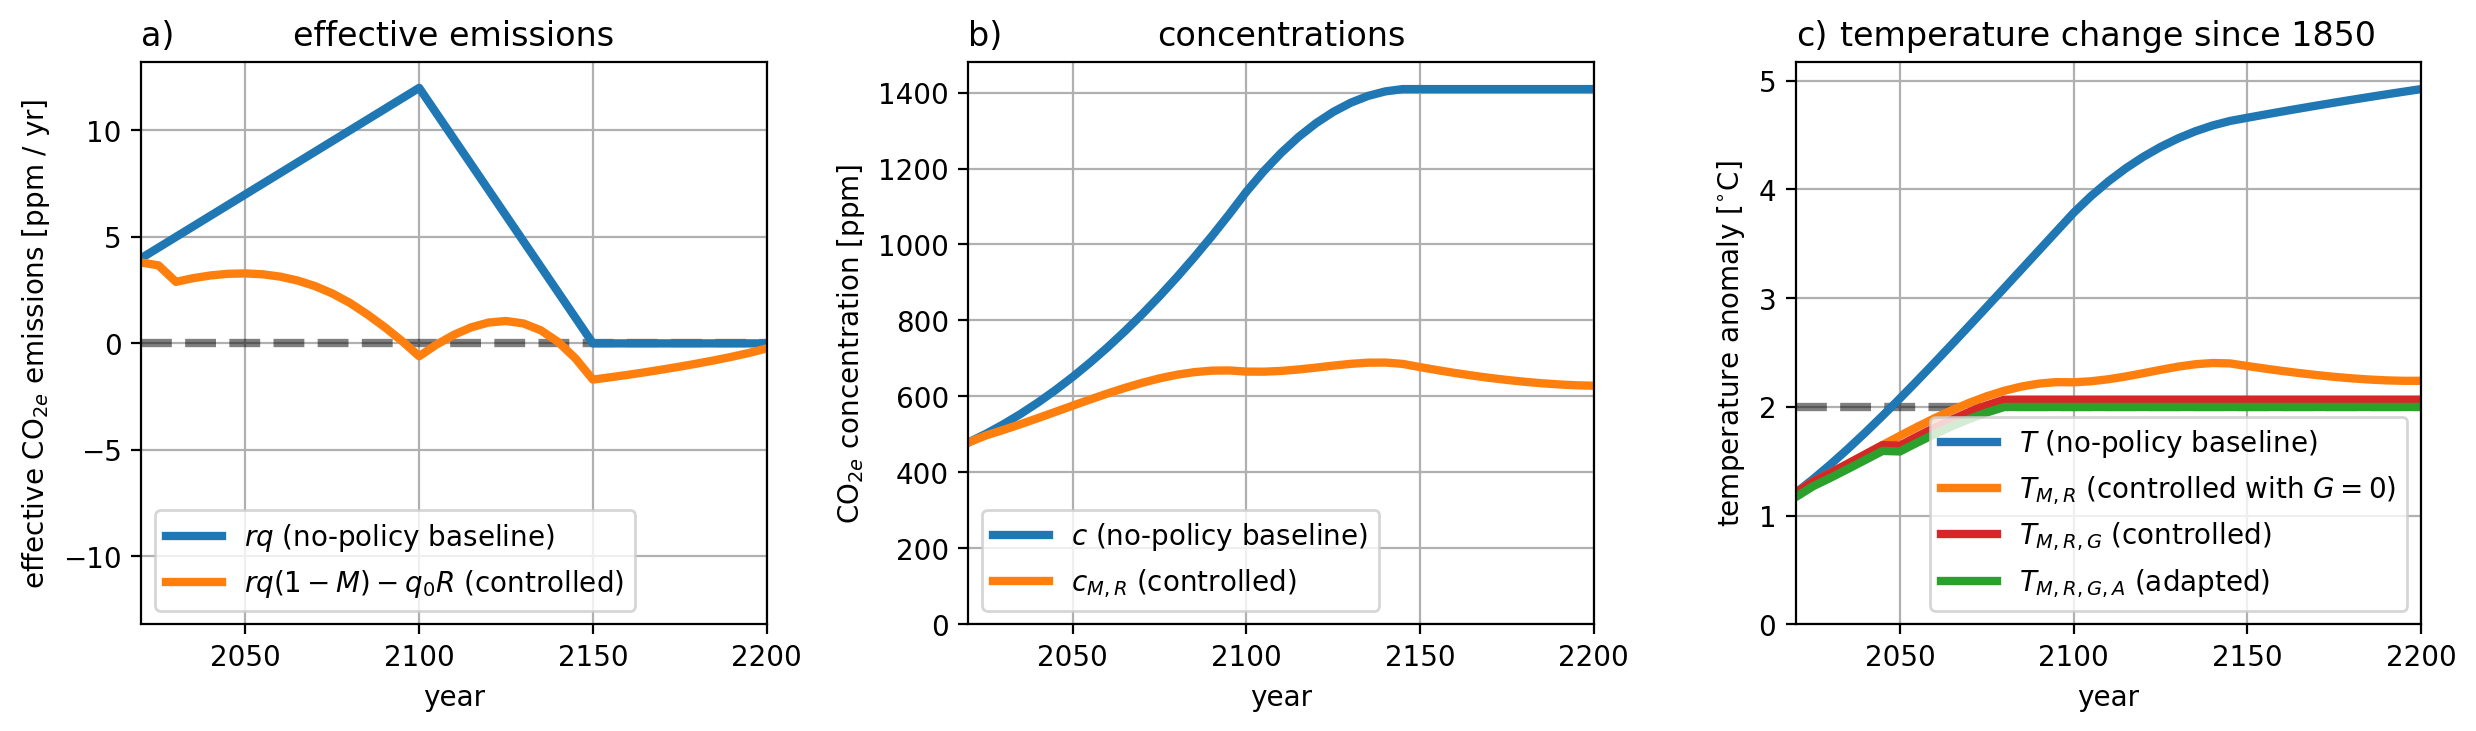
\includegraphics[width=1.0\textwidth]{figures/default-temp_carbon_and_temperatures.png}
\centering
\caption{}
\label{fig.temp_and_carbon}
\end{figure}

\subsection{Temperature response to CO$_{2}$ forcing}
The evolution of the global-mean near-surface temperature anomaly (relative to the initial time $t_{0} = 2020$) is determined by the two-box linear energy balance model \citep[e.g][]{gregory_vertical_2000, held_probing_2010}:
\begin{gather}
    C_{U} \dv{T'}{t} = -B T' - \kappa( T' - T_{D}') + F'(t), \label{eq.upper_ocean}
    \\
    C_{D} \dv{T_{D}'}{t} = \kappa (T' - T_{D}'),\label{eq.deep_ocean}
\end{gather}
where (\ref{eq.upper_ocean}) represents the upper ocean with average temperature anomaly $T'$, and (\ref{eq.deep_ocean}) represents the deep ocean with an average temperature $T_{D}'$. The near-surface atmosphere exchanges heat rapidly with the upper ocean and thus the global-mean near-surface air temperature is also given by $T'$. The model parameters are: the upper ocean heat capacity $C_{U}$ (including a negligible contribution $C_{A} \ll C_{U}$ from the atmosphere); the deep ocean heat capacity $C_{D}$; the climate feedback parameter $B$; the ocean mixing rate $\kappa$; and $F'(t)$ the anomalous anthropogenic radiative forcing. We hereafter drop the $'$ when denoting anomalies for convenience.

If the forcing $F(t)$ varies on timescales longer than the fast relaxation timescale $\tau_{U} = C_{U}/(B + \kappa)$ then we can ignore the time-dependence in the upper ocean and approximate
\begin{equation}
    T \approx \frac{F+\kappa T_{D}}{B + \kappa},
    \label{eq.shallow_approx}
\end{equation}
where the evolution of the deep ocean
\begin{equation}
    C_{D} \dv{T_{D}}{t} \approx - \frac{B \kappa}{B + \kappa} T_{D} + \frac{\kappa}{B + \kappa} F
    \label{eq.deep_ode}
\end{equation}
occurs on a slower timescale $\tau_{D} \equiv \dfrac{C_{D}}{B} \dfrac{B + \kappa}{\kappa}$. Plugging the exact solution to (\ref{eq.deep_ode}) into (\ref{eq.shallow_approx}) gives
\begin{equation}
    T(t) = \frac{F(t)}{B + \kappa} + \frac{\kappa}{B} \frac{1}{(B+\kappa)} \int_{t_{0}}^{t} \frac{ e^{-(t-t')/\tau_{D}}}{\tau_{D}} F(t') \, \text{d}t'.\label{eq.temperature}
\end{equation}
We identify the first term in (\ref{eq.temperature}) as the transient climate response \citep{gregory_transient_2008}, which dominates for $t-t_{0} \ll \tau_{D}$ while the second term is a slower ``recalcitrant" response due to a weakening of ocean heat uptake as the deep ocean comes to equilibrium with the transiently warmer upper ocean \citep{held_probing_2010}. While the contribution of the recalcitrant component to historical warming is thought to be small (justifying our initial condition of $T' = T = \SI{0}{K}$), it contributes significantly to 21st century and future warming, especially when the instantaneous radiative forcing remains plateaus or vanishes completely $F(t) \rightarrow 0$ and the recalcitrant component is the only remaining cause of temperature change \citep{gregory_transient_2008, held_probing_2010}.

The behavior of the model on short and long timescales is illustrated by applying it to the canonical climate change experiment in which CO$_{2}$ concentrations increase at 1\% per year until doubling. The temperature anomaly first rapidly increases until it reaches the Transient Climate Sensitivity $TCS = \dfrac{F_{2\times}}{B + \kappa}$ around the time of doubling $t=t_{2\times}$ (with $t_{2\times} - t_{0} \ll \tau_{D}$) and then gradually asymptotes to the Equilibrium Climate Sensitivity $ECS = \dfrac{F_{2\times}}{B} > TCS$ on a much longer timescale $t-t' \gg \tau_{D}$.

The evolution of the controlled temperature anomaly
\begin{equation}
    T_{M,R,G}(t) = \frac{F_{M,R,G}(t)}{B + \kappa} + \frac{\kappa}{B} \frac{1}{(B+\kappa)} \int_{t_{0}}^{t} \frac{ e^{-(t-t')/\tau_{D}}}{\tau_{D}} F_{M,R,G}(t') \, \text{d}t'\label{eq.temperature}
\end{equation}
is thus driven by the controlled net radiative forcing $F_{M,R,G}$.

\subsection{Climate damages}

Annual climate damages are assumed to be of the quadratic form $D(t) = \beta T(t)^{2}$, such that successive temperature increases are increasingly damaging, based on empirical estimates of damages which range from linear to cubic functions of global-mean temperature \citep{stern_economics_2007}. The default value of the damage parameter $\beta$ is chosen to be roughly similar to the DICE model for low levels of warming \citep{nordhaus2013dice}, resulting in damages of 2\% of global world product at \SI{2}{\celsius}. \textbf{A}daptation to climate change impacts (e.g. building sea walls, installing air conditioning units, planting climate-resilient crops) is parameterized by reducing annual damages by a fraction $A(t) \in [0,1]$, such that the total controlled damages are:
\begin{equation}
    D_{M, R, G, A} = \beta \; (T_{M, R, G}(t))^{2} \; (1-A(t)).
\end{equation}

\subsection{Control costs}

The annual costs of climate control technologies are given by
\begin{equation}
    \mathcal{C}_{M, R, G, A}(t) = \sum_{\alpha \in \mathcal{A}} \mathcal{C}_{\alpha} f(\alpha(t)),
\end{equation}
where $\mathcal{A} = \{M, R, G, A \}$ is the set of climate control technologies considered here, $\mathcal{C}_{\alpha}$ is the reference cost of each climate control technology, and $f(\alpha)$ is a function that determines how the deployment cost increases as a function of fractional deployment. The reference cost corresponds to the hypothetical cost of full deployment of that technology (e.g. $C_{G}$ is the cost of offsetting all potential warming since preindustrial with geoengineering, including both direct costs and damages due to side effects), but it may be more usefully tuned based on a smaller deployment threshold, such as 25\%, for which costs estimates are likely to be more reflective of both plausible short-term deployment fractions and costs. Here, we will focus on the medium deployment cost scenario $f(\alpha) = \alpha^{2}$, which has the following convenient properties: 
\begin{itemize}
    \item $\left. \dv{f}{\alpha}\right|_{\alpha=0} = 0$ (initial marginal deployment is effectively free)
    \item $f(1) = 1$ (full deployment costs $\mathcal{C}_{\alpha}$), and
    \item $\dv[2]{f}{\alpha} > 0$ (convex, such that deployment gets progressively more and more expensive).
\end{itemize}

\subsection{Optimization Methods}

We use the Interior Point Optimizer (\href{https://github.com/coin-or/Ipopt}{https://github.com/coin-or/Ipopt}), an open source software package for large-scale nonlinear optimization, to minimize the various objective functions subject to assumed policy constraints, as described in Section \ref{sec.policy_frameworks}. In practice, the control variables $\mathcal{A} = \{ M, R, G, A\}$ and diagnostics $c(t)$, $T(t)$, $D(t)$, and $\mathcal{C}$ are discretized into $N$ timesteps (default $\Delta t = \SI{10}{years}$) resulting in an $4N$-dimensional optimization problem. In the default (deterministic and convex) configuration, the model takes only $\mathcal{O}(\SI{10}{ms})$ to solve after just-in-time compiling and effectively provides user feedback in real time, making it amenable to our forthcoming interactive web application (e.g. following the lead of the impactful \href{https://en-roads.climateinteractive.org/scenario.html?v=2.7.11}{En-ROADS} model, \citealt{siegel2018roads}).

\section{Climate change policy frameworks}\label{sec.policy_frameworks}

In contrast to conventional Integrated Assessment Models, which follow classic economic theories of optimal economic growth and solve for the maximal welfare based on the discounted utility of consumption, we here completely ignore economic feedbacks and simply aim to minimize the costs– and maximize the benefits– of deploying climate change controls, subject to constraints from policy goals.

In Section \ref{sec.cost_benefit}, we describe a cost-benefit analysis approach which finds the trajectories of control deployments that optimize trade-offs between the costs of deploying climate controls and the benefit of avoiding climate damages due to these controls. The cost-benefit approach depends strongly on the magnitude of the poorly-constrained damage function $D(T)$, which is thought to be under-estimated by conventional bottom-up approaches \citep{ackerman_limitations_2009}. Thus, in Section \ref{sec.paris_goal} we also explore an alternative scenario in which we instead impose an upper bound goal on climate damages (as in the 2015 United Nations Paris Agreement on Climate Change) and find the lowest cost climate control trajectories which still satisfy this constraint.

\subsection{Approach 1: Cost-benefit analysis}\label{sec.cost_benefit}

A common economic assumption is that society discounts future costs and benefits relative to present by a multiplicative factor $(1 + \rho)^{-(t-t_{0})}$, determined by the utility discount rate $\rho$ \citep[e.g. see reviews in][]{broome_discounting_1994, stern_economics_2007}. Ethical justifications for such a non-zero discount rate are controversial and unconvincing \citep{ramsey_mathematical_1928, solow_economics_1974, stern_economics_2007} and so here we set $\rho = 0$ as our default discount rate in the spirit of inter-generational equity\footnote{Following \cite{stern_economics_2007}'s discussion of the discount rate $\rho = \eta \frac{\dot{c}}{c} + \delta$, we argue against the use of a \textit{social discount rate} on ethical terms \citep{ramsey_mathematical_1928, solow_economics_1974}, setting $\eta \frac{\dot{c}}{c}=0$, and argue that the \textit{pure time discount rate}, the time decay rate of the probability that society exists, is small $\delta \approx 0$, such that $\rho \approx 0$. We note that while a discount rate of zero introduces a sensitivity to the length of the time period considered, the conventional use of discount rates results in an even more absurd assertion that future generations are worthless.}. 

Here, we interpret the cost $\mathcal{C}$ of climate change as the cost of deploying climate controls to reduce climate damages while the benefits $\mathcal{B}$ are the avoided climate damages. A straight-forward solution of the cost-benefit problem is thus to minimize the difference between the time-integrated (potentially discounted) costs and benefits:
\begin{align}
    &\min \left\{ \sum_{t_{0}}^{t_{f}} 
    \left(\mathcal{C}_{M, R, G, A} - \mathcal{B}_{M, R, G, A}\right) (1 + \rho)^{-(t-t_{0})} \right\} \\
    = \; & \min \left\{ \sum_{t_{0}}^{t_{f}} \left( \sum_{\alpha \in \mathcal{A}} \mathcal{C}_{\alpha} f(\alpha(t)) + \beta (T_{M, R, G})^{2}(1-A(t)) \right) (1 + \rho)^{-(t-t_{0})} \right\}
\end{align}



\subsection{Approach 2: Cost-effectivness of avoiding probabilistic damage thresholds (i.e. Paris Agreement)}\label{sec.paris_goal}

\begin{figure}[htb!]
\noindent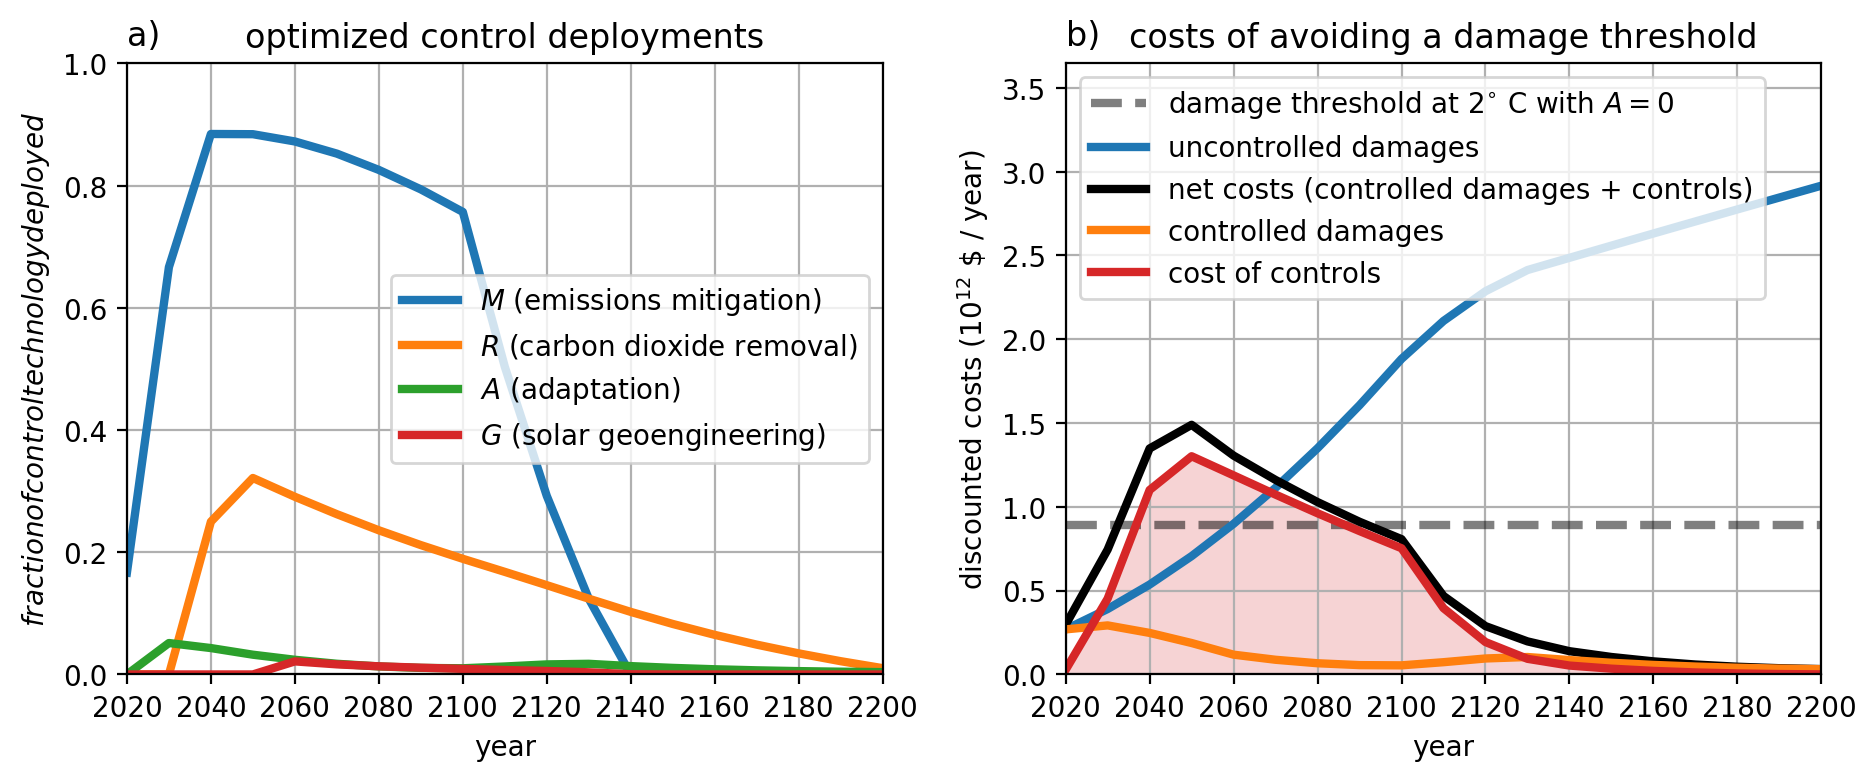
\includegraphics[width=1.0\textwidth]{figures/default-temp_controls_and_damages.png}
\centering
\caption{}
\label{fig.approach2}
\end{figure}

\subsection{Designing reactive climate policy for an uncertain future}

\section{Qualitative model results}

\subsection{Multiple climate controls are better than one}

\subsection{Uncertainty in climate damages strengthens the case for early action}

\subsection{Optimal policy is as arbitrary as the discount rate}

\section{Discussion}

%\appendix{Comprehensive formulation of optimization problems}

\bibliographystyle{apalike}
%\bibliographystyle{unsrtnat}
\bibliography{references.bib, refs_by_hand.bib}

\end{document}